% Creation
\section{Creation}
\subsection{Storing the project}
\begin{frame}{Storing the project}
    \begin{figure}
        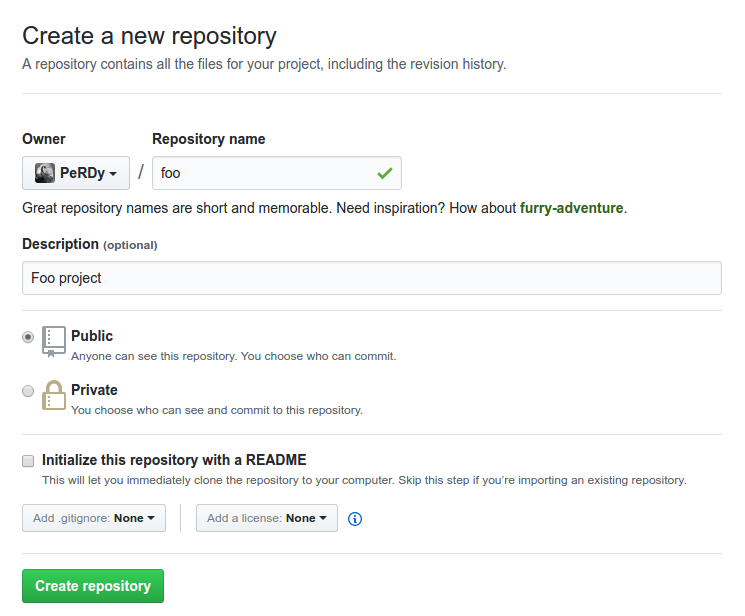
\includegraphics[width=\textwidth,height=0.8\textheight,keepaspectratio]{create_repository.png}
    \end{figure}
    \note{
        Esta charla está completamente orientada a open source así que, ¿por qué no trabajar con GitHub?
    }
\end{frame}

\subsection{Create the project skeleton}
\begin{frame}[fragile]{Create the project skeleton}
    \begin{block}{Cookiecutter context}
        Define all variables needed by cookiecutter to properly create the project skeleton, these variables can be found in \textit{cookiecutter.json} file.
    \end{block}
    \pause
    \begin{block}{Create skeleton}
        Execute cookiecutter with previously defined context to create the project skeleton.
    \end{block}
    \pause
    \begin{block}{Commit \& push}
        Time to do your first commit and push to repository:
        \begin{minted}{bash}
git remote add origin git@github.com:PeRDy/foo.git
git commit -a -m "Initial commit"
git push
        \end{minted}
    \end{block}
    \note {
        Para crear el proyecto:
        \begin{enumerate}
            \item Definir el contexto necesario para Cookiecutter: nombre, autor, repositorio...
            \item Crear el esqueleto del proyecto con la plantilla.
            \item Commit iniciar y pushear.
        \end{enumerate}
    }
\end{frame}

\subsection{Project hierarchy}
\begin{frame}{Project hierarchy}
    \begin{columns}
        \begin{column}{0.2\textwidth}
            \begin{figure}
                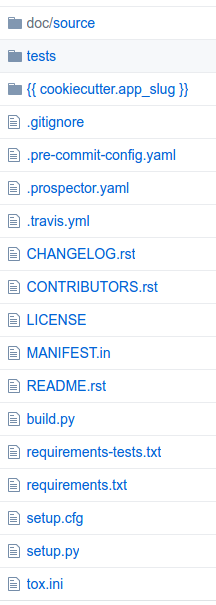
\includegraphics[width=\textwidth,height=\textheight,keepaspectratio]{project_skeleton.png}
            \end{figure}
        \end{column}
        \begin{column}{0.80\textwidth}
            \begin{block}{Documentation folder}
                The place that keeps all the documentation source files as well as the doc config file.
            \end{block}
            \pause
            \begin{block}{Tests folder}
                All tests files are stored in a tests folder where tests collectors can gather them without problems.
            \end{block}
            \pause
            \begin{block}{Application folder}
                The application itself, the \emph{python package} distributed, and the same that other users will import in their applications.
            \end{block}
            \pause
            \begin{block}{Root files}
                Files that keeps in the root directory are usually:
                \begin{itemize}
                    \item Tools configuration.
                    \item Services configuration.
                    \item Build scripts.
                    \item Metadata.
                \end{itemize}
            \end{block}
        \end{column}
    \end{columns}
    \note{
        \begin{description}
            \item[Configuración de herramientas] Prospector, Pre-commit, Git.
            \item[Configuración de servicios] Travis.
            \item[Scripts de construcción] \texttt{build.py}, \texttt{setup.py}, \texttt{tox.ini}.
            \item[Metadatos] Readme, manifest, contributors, changelog, requirements, \texttt{setup.cfg}.
        \end{description}
    }
\end{frame}

\begin{frame}[fragile]{Relevant files I}
    \begin{block}{Manifest}
        This file, \texttt{MANIFEST.in}, with own syntax\footnote[1]{\href{https://docs.python.org/3/distutils/commandref.html#sdist-cmd}{https://docs.python.org/3/distutils/commandref.html#sdist-cmd}} defines the directories and files that will be included in the distributable package.
    \end{block}
    \pause
    \begin{block}{Requirements}
        List all requirements of your project, that are added as dependencies when installed. Usually requirements are splitted in two files: \texttt{requirements.txt} for real dependencies and \texttt{requirements-tests.txt} for dependencies necessaries to test the project.
    \end{block}
    \pause
    \begin{block}{Metadata}
        Metadata files: \texttt{README.rst}, \texttt{CONTRIBUTORS.rst}, \texttt{CHANGELOG.rst} and \texttt{LICENSE}.
    \end{block}
    \note{
        El fichero README puede ser escrito en reStructuredText o en Markdown. Este fichero, renderizado, será la página principal del proyecto en GitHub,
    }
\end{frame}

\begin{frame}{Relevant files II}
    \begin{block}{Tools and Services config}
        Configuration files for tools and services: \texttt{setup.cfg}, \texttt{.pre-commit-config.yaml}, \texttt{.prospector.yaml}, \texttt{.travis.yml}, \texttt{.gitignore}.
    \end{block}
    \pause
    \begin{block}{Setup}
        Main file that defines how the project will be packaged, gather metadata from other files and provides an interface to create distributable packages.
    \end{block}
    \pause
    \begin{block}{Tox}
        Tox file, \texttt{tox.ini}, defines the environments and commands that tox executes. In this case, defines an environment for each python version that should be tested, another for run lint tools and the last one for compile documentation.
    \end{block}
    \note{
        El fichero principal de configuración es \texttt{setup.cfg}, que es un fichero de estilo \texttt{.ini}, dividido en secciones con configuraciones para las diferentes herramientas como por ejemplo \emph{bumpversion}, \emph{pytest} y \emph{coverage}.

        El fichero \texttt{setup.py} contiene la versión actual del proyecto, su nombre y su lista de requirements.

        Tox está integrado con Travis.
    }
\end{frame}
\begin{frame}{Relevant files III}
    \begin{block}{Build}
        The build file, \texttt{build.py}, is the entrypoint for everything related to build, including \emph{testing}, \emph{packaging} and \emph{distributing}. This is a command line application using \emph{Clinner} that provides a set of utility commands such as:
        \begin{itemize}
            \item Run tests and code coverage.
            \item Run lint.
            \item Run tox.
            \item Create documentation.
            \item Upgrade version, create package and upload to pypi.
        \end{itemize}
    \end{block}
    \note {
        Estas son las funciones del script de Clinner, más adelante se muestra la salida de la ayuda del script.
    }
\end{frame}
